% $Header$
% $Author$
% $Date$
% $Revision$
% $Log$
% Revision 1.3  2005/02/22 07:31:00  fager
% Corrections from M.Kelly implemented
%
% Revision 1.2  2004/10/21 18:59:06  fager
% Version logging added. Comments from KA and MK implemented.
%

\documentclass[10pt,a4paper]{article}
\usepackage{amssymb}
\usepackage{times}
\usepackage{graphicx}
%\usepackage{hyperref}

\newcommand{\figref}[1]{Fig.~\ref{fig:#1}}
\newcommand{\Figref}[1]{Fig.~\ref{fig:#1}}
\newcommand{\appref}[1]{Appendix~\ref{app:#1}}
\newcommand{\Appref}[1]{Appendix~\ref{app:#1}}
\newcommand{\tabref}[1]{Table~\ref{tab:#1}}
\newcommand{\Tabref}[1]{Table~\ref{tab:#1}}
\newcommand{\equref}[1]{(\ref{equ:#1})}
\newcommand{\Equref}[1]{Equation (\ref{equ:#1})}
\newcommand{\refref}[1]{\cite{#1}}
\newcommand{\secref}[1]{section~\ref{sec:#1}}
\newcommand{\Secref}[1]{Section~\ref{sec:#1}}

\newcommand{\matlab}{\textsc{Matlab\,}}

\setcounter{secnumdepth}{3} \setcounter{tocdepth}{3}

\title{MATLAB Milou Toolbox \\ User's Guide}
\author{Christian Fager\\christian.fager@mc2.chalmers.se}
\begin{document}
\maketitle %\pagebreak
\tableofcontents
% $Header$
% $Author$
% $Date$
% $Revision$
% $Log$
% Revision 1.2  2004/10/21 18:59:06  fager
% Version logging added. Comments from KA implemented.
%
\section{Introduction}%\hypertarget{Introduction}
The \emph{Matlab-Muwave toolbox}\footnote{Muwave is hereafter used
as a short-hand notation for the \matlab-Muwave toolbox.} is a
collection of functions to facilitate easy handling of
S-parameters in the \matlab\footnote{\matlab is a trademark of The
Mathorks Inc., Natick,MA, U.S.A} environment. The computational
power and programming framework of \matlab can thereby be applied
to calculations involving measured or simulated data. This makes
it particularly suited for device modelling applications, for
which e.g. CAD tools are of limited use.

The purpose of this document is to describe the basic
functionality offered by the toolbox in order for new users to get
started and acquainted to the most commonly used functions.

\subsection{Further help}
For a more detailed description of each function encountered in
this text, users are referred to the Matlab-Muwave Reference manual
and on-line help provided by typing \verb">> help <command name>"
or \verb">> helpwin <command name>" at the \matlab command prompt.
It is, however, assumed that readers of this document are
reasonably familiar with the general \matlab environment.

\subsection{Feedback}
Muwave is under continuous development. Most certainly you will
find bugs and annoying inconsistencies as you start using it. It
is therefore of great help for us to get feedback on features that
are missing or if errors are found. Therefore, please do not
hesitate to contact us if you have anything you are wondering
about, report errors you have found, or if you have developed your
own functionality that you want to share.

\vspace{5mm} \setlength{\tabcolsep}{0.5cm} \noindent
\begin{center}
    \begin{tabular}{ll}
    Kristoffer Andersson & Christian Fager\\
    kristoffer.andersson@chalmers.se &
    christian.fager@chalmers.se\\
\end{tabular}
\end{center}

% $Header$
% $Author$
% $Date$
% $Revision$
% $Log$
% Revision 1.2  2004/10/21 18:59:06  fager
% Version logging added. Comments from KA implemented.
%
\section{Installation}%\hypertarget{Installation}
Milou has been developed using \matlab v.6.5 (Release 13), which
is assumed to be installed on the user's computer. Please check
the Help/About menu to make sure you are running this or a later
version.

The installation of the Milou-toolbox consists of a few simple
steps:
\begin{enumerate}
    \item Download the latest version from the Milou web page at \newline http://www.mc2.chalmers.se/mc2/mel/edu/g\_courses/emp\_mod/milou/.
    \newline The downloaded zip-file contains all \matlab m-files and
documentation necessary.
    \item Extract all files to a directory of your choice. In WinZip, make
    sure to have the ''Use folder names'' option checked.
    \item Add Milou to \matlab's path. This is done from the
    File menu by selecting ''Set Path...''. Click ''Add Folder''
    in the dialog box that appears and browse to select the ''matlab\_milou''
    directory, which was created where you extracted the
    zip-file. Please make sure to press the ''Save button''
    before closing the Set Path dialog box.
    \item Normally, Milou is now ready for action. However, it
    may in rare cases be necessary to execute the following line before
    Milou is used the first time:
    \begin{verbatim}
        >> clear classes; rehash;
    \end{verbatim}
\end{enumerate}
You can verify that Milou has been successfully installed by
creating an empty measurement object. This is done by executing:
\verb">> meassp". The following should be displayed at the command
prompt:
\begin{verbatim}
    >> meassp
    Measurement info
        Date : 18-Oct-2004 20:33:57
        Origin :
        Operator :
        Info :
    Measurement state
        MeasType:   SP
    Measurement Data
    xparam-object
        type:  S
        reference: 50
        ports: 2
        elements:  0
\end{verbatim}

% $Header$
% $Author$
% $Date$
% $Revision$
% $Log$
% Revision 1.2  2004/10/21 18:59:06  fager
% Version logging added. Comments from KA implemented.
%

\section{Muwave data hierarchy} %\hypertarget{hierarchy}
Before describing how to use it, some effort will be spent on
briefly explaining the data structure used to store measurement
data in Muwave.

\subsection{Overview}
A typical S-parameter measurement is in the form of 2-by-2 complex
matrices versus $n$ frequency points. Most calculations such as
gain, impedance, and stability are then carried out on a
``per-frequency'' basis.

The way in which Muwave stores this data is a complex three
dimensional ($2 \times 2\times n$) matrix. \matlab, however, has
no built in functionality to perform operations in this
manner---it simply does not understand along which dimensions it
should perform the operations.

Muwave, however, uses the object-oriented capabilities offered by
\matlab to define a low-level \emph{S/Y/Z/T-parameter data class},
for which all common \matlab operations, such as *, +, -, /, ./
etc. have been redefined to operate ``per-frequency''. On a higher
level, an \emph{S-parameter measurement class} has been defined,
which handles information about the frequencies, the bias
settings, the measurement file source, etc. All these properties
are automatically populated by parsing the measurement files when
read into \matlab.

\Figref{ClassHierarchy} shows an overview of the different Muwave
classes implemented, and their respective purpose. A short
description of each of them is given below.

\begin{figure}[htbf]
  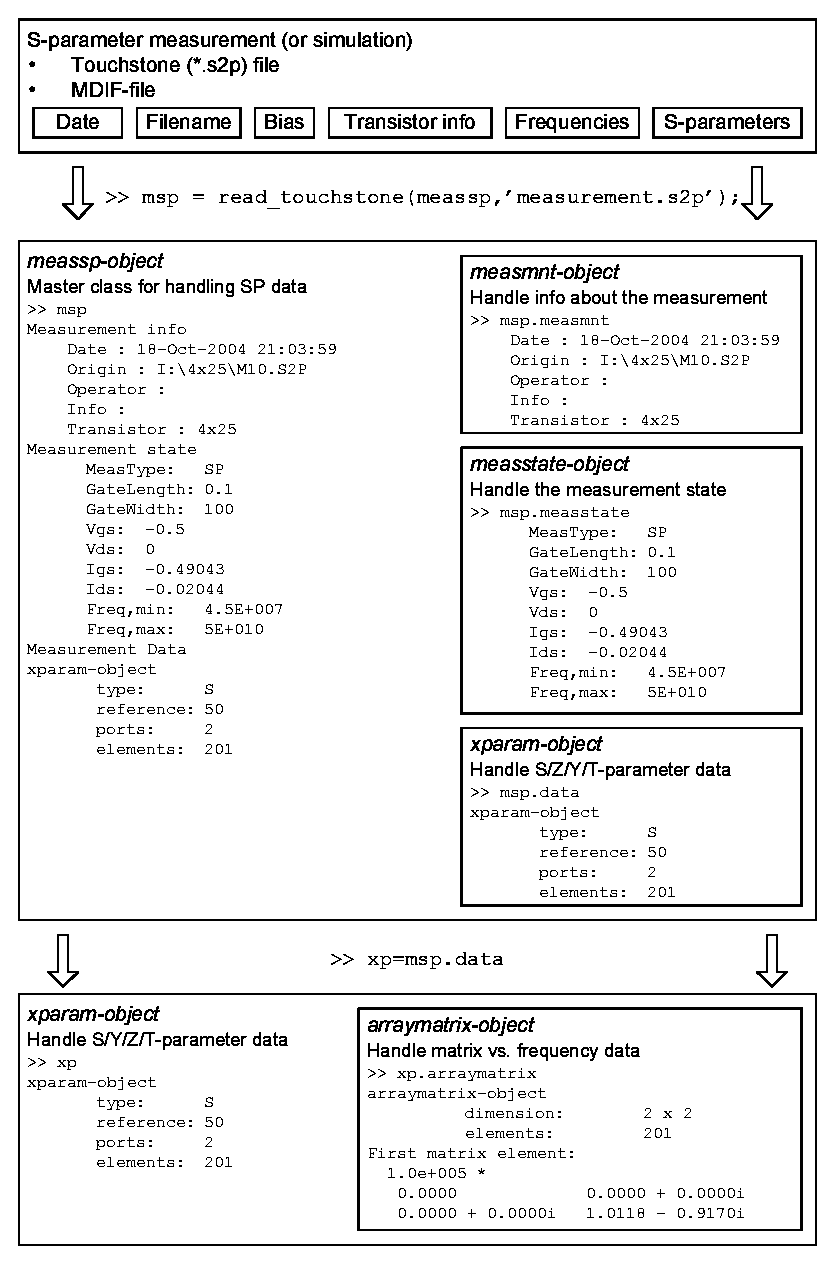
\includegraphics[width=\textwidth]{Figures/ClassOverview3.eps}
  \caption{Overview of the Muwave class hierarchy.}\label{fig:ClassHierarchy}
\end{figure}

\subsection{meassp}
\emph{meassp} is the top level class for handling S-parameters.
All functions for reading single measurement files generate
meassp-objects. The resulting measurement information is then
contained its three sub-classes: \emph{measmnt}, \emph{measstate},
and \emph{xparam}.

\subsection{measmnt}
\emph{measmnt} is intended to store information about the
measurement. This can typically include date of measurement, the
measurement operator, the file origin, the transistor type etc.

\subsection{measstate}
\emph{measstate} contains numerical data describing the
measurement conditions. Typically, this is gate bias voltage,
drain current, gate width, pulse length, temperature,
etc.

\subsection{xparam}
\emph{xparam} contains the actual S-parameter data and the corresponding frequencies. 
Or, in fact, it can be data of either S, Y, Z, or T-type. The class keeps track
of which type of data it contains and has built in functionality
to convert between them. Moreover, it stores the reference
impedance so that S-parameters may be converted to other
impedances if required. The numerical complex S/Y/Z/T-data is
stored in an \emph{arraymatrix} object.

\subsection{arraymatrix}
\emph{arraymatrix} is the low level class that is used to
implement matrix multiplication, inversion, conjugate transpose,
addition etc. ``per frequency'', as is needed e.g. for conversion
between Z- and S parameters.

\subsection{Additional classes}
In addition to the classes described above, there exists also a
few other classes that handle sweeps of measurements and
model/netlist generation. These are described later in
\secref{sweeps} and \secref{mna}, respectively.

% $Header$
% $Author$
% $Date$
% $Revision$
% $Log$
% Revision 1.2  2004/10/21 18:59:06  fager
% Version logging added. Comments from KA implemented.
%
\section{Reading and storing single measurement files}
The easiest and best way to introduce the functionality of MuWave
is probably by an example. The example measurement used here is
for an InP-HEMT device biased in the active region. The
measurement is stored as a TouchStone file at: \newline
\verb"muwave/test/d0509/d0509_20".

\subsection{The TouchStone file format}
The most commonly used file format for storing S-parameter files
is the TouchStone format\footnote{TouchStone is a registered
trademark of Agilent Corporation. A complete specification of the
file format can be found in either
www.eda.org/pub/ibis/connector/touchstone\_spec11.pdf or the
Agilent ADS manual.}. These files are typically identified by a
.S2P file extension (although not the case for the example file
above), where 2 denotes the number of ports in the measurement
data. Below is shown an example of how the first couple of lines
of a Touchstone file typically look like:
\begin{small}
\begin{verbatim}
    !Date: 2002-10-25, 08:50

    !Vgs = -1.000000E-1
    !Vds = 1.500000E+0
    !Ig = -2.784000E-7
    !Id = 1.974500E-2

    #HZ S RI R 50
    1.000000E+9 9.921265E-1 -6.970215E-2 -3.964478E+0 ...
    1.490000E+9 9.887085E-1 -1.027222E-1 -3.976196E+0 ...
    1.980000E+9 9.827881E-1 -1.362915E-1 -3.920410E+0 ...
    2.470000E+9 9.783020E-1 -1.674194E-1 -3.943237E+0 ...
    2.960000E+9 9.721069E-1 -1.990662E-1 -3.927979E+0 ...
        ...
\end{verbatim}
\end{small}
Rows starting with exclamation marks (!) indicate comments, but
are here used to store additional information about the
measurements. In this case, which is typical, the comments reveal
the biasing conditions as well as the date of measurement.

The next important section is the line starting with \verb"#".
This line reveals the format of the following data. First on that
line, \verb"HZ" is written to indicate that the first column of
the data, which is always the frequency, is given in Hertz.
Thereafter indicates \verb"S" that the data is indeed S-parameter
data. The following \verb"RI" tells us that the S-parameters are
given in ``$\mathrm{Re}(S)~\mathrm{Im}(S)$'' format. Other
alternatives are \verb"MA" and \verb"DB", corresponding to
``$|S|~\angle S$'' and ``$20 log_{10}(|S|)~\angle S$'',
respectively. Finally, \verb"R 50" indicates that the S-parameters
are given for a $50 \Omega$ system impedance. The remainder of the
file consists of lines in the following format:
\begin{small}
\begin{verbatim}
    freq real(S11) imag(S11) real(S21) imag(S21) real(S12)...
\end{verbatim}
\end{small}
where in this case the \verb"RI" format has been assumed.

\subsection{read\_touchstone}
The \verb"read_touchstone" function allows a straightforward way
of importing TouchStone files into MuWave:

\begin{small}
\begin{verbatim}
    >> msp = read_touchstone(meassp,'muwave/test/d0509/d0509_20')
    Measurement info
        Date : 2002-10-25, 08:50
        Origin : muwave/test/d0509/d0509_20
        Operator :
        Info :
    Measurement state
    	MeasType:	SP
    	Vgs:	-0.1
    	Vds:	1.5
    	Igs:	-2.784e-007
    	Ids:	0.019745
    xparam-object
    	 type:	S
    	 reference:	50
    	 ports:	2
    	 elements:	101
    	 freq:	1E+009 -> 5E+010
\end{verbatim}
\end{small}

The variable \verb"msp" is now an instance of an \verb"meassp"
object, as illustrated in \figref{ClassHierarchy}. The parameters
displayed indicate that \verb"read_touchstone" has parsed the
header in the TouchStone file and put the information in the
corresponding sub-objects. The following sections will describe
how to access and manipulate these parameters and properties.

\subsection{write\_touchstone}
Naturally, it is also possible to store a \verb"meassp" object as
a TouchStone file. The syntax is similar as for
\verb"read_touchstone":
\begin{small}
\begin{verbatim}
    >> write_touchstone(msp,'c:\users\nn\temp\datatest.s2p');
\end{verbatim}
\end{small}

% $Header$
% $Author: fager $
% $Date: 2004-10-21 20:59:19 +0200 (Thu, 21 Oct 2004) $
% $Revision: 223 $
% $Log$
% Revision 1.2  2004/10/21 18:59:06  fager
% Version logging added. Comments from KA implemented.
%
\section{Basic access and manipulation of properties}\label{sec:DACManip}
Once the measurement data has been read into an \verb"meassp"
object, there are several methods implemented to access and
manipulate their contents.

First, it will be described how to access and manipulate the
\verb"measstate" and \verb"measmnt" object properties. The
S-parameter data, which is stored in an \verb"xparam" object is
treated separately in \secref{SPMod}.

\subsection{set and get}
Generally, the two functions \verb"set" and \verb"get" are used to
manipulate and access the properties of an \verb"meassp" object.
It is important to note that these functions can be applied
directly to the \verb"meassp" object, although the property that
is being accessed is in fact member of the \verb"measmnt" or
\verb"measstate" sub-classes. A typical usage of them is shown
below:

\begin{small}
\begin{verbatim}
    >> msp = read_touchstone(meassp,...
        'matlab_milou/test/d0509/d0509_20');
    >> get(msp,'Date')
    ans =
    2002-10-25, 08:50

    >> get(msp,'Ids')
    ans =
        0.0197

    >> get(msp,'Freq')
    ans =
    1.0e+010 *
        0.1000
        0.1490
        ...

    >> msp = set(msp,'Operator','Tintin','Igs',1,...
        'Date',datestr(now))
    Measurement info
        Date : 19-Oct-2004 15:28:00
        Origin : matlab_milou\test\d0509\d0509_20
        Operator : Tintin
        Info :
    Measurement state
        MeasType:   SP
        Vgs:    -0.1
        Vds:    1.5
        Igs:    1
        Ids:    0.019745
        Freq,min:   1E+009
        Freq,max:   5E+010
    Measurement Data
    xparam-object
        type:  S
        reference: 50
        ports: 2
        elements:  101
\end{verbatim}
\end{small}

\subsection{The dot-operator}
A more convenient way of accessing and manipulating \verb"meassp"
data than using \verb"set" and \verb"get" is to use the ``dot''-
operator. The following expressions are equivalent and illustrate
the principle of operation:

\begin{small}
\begin{verbatim}
    >> msp = set(msp,'Operator','Phyllis');
    >> msp.Operator = 'Phyllis';

    >> f = get(msp,'Freq');
    >> f = msp.Freq;
\end{verbatim}
\end{small}

The dot-assignments above automatically call the
\verb"@meassp/subsasgn.m" function, which overloads the built-in
\verb"subsasgn" function that is used to handle the dot-operator
for other input types. See \verb">> help subsasgn" for further
details. Similar to \verb"get", \verb"subsref" plays the same role
when the dot-operator is used to access a parameter value.

\subsection{Adding a property}
It is sometimes required to add a property that was not defined in
the TouchStone file. For example, we might want to add a
\verb"VNA" property that we can use to identify which VNA was used
during the measurements. The procedure to add a
\verb"measmnt"-property is easy:

\begin{small}
\begin{verbatim}
    >> msp = addprop(msp,'VNA','HP 8510C')
    Measurement info
        Date : 2002-10-25, 08:50
        Origin : matlab_milou\test\d0509\d0509_20
        Operator :
        Info :
        VNA : HP 8510C
        ...
\end{verbatim}
\end{small}
To add a \verb"measstate" property, the procedure is a bit
different. First, the \verb"measstate" object must be extracted
from the \verb"meassp" object. The new property can then be added
to the \verb"measstate" object. This modified \verb"measstate"
object should then be put back into the original \verb"meassp"
object. It is maybe more easy to understand in code:

\begin{small}
\begin{verbatim}
    >> mstate = get(msp,'measstate');
    >> mstate = addprop(mstate,'Temp',75);
    >> msp = set(msp,'measstate',mstate)
    ...
    Measurement state
        MeasType:   SP
        Vgs:    -0.1
        Vds:    1.5
        Igs:    -2.784E-007
        Ids:    0.019745
        Freq,min:   1E+009
        Freq,max:   5E+010
        Temp:   75
    ...
\end{verbatim}
\end{small}

\subsection{Reduction and extension of frequency range}
Another operation that is commonly encountered is to remove
undesired frequencies, or to reduce the number of frequency
points. Two methods can be used.

The first case applies when the frequencies remain the same, but
some points should be removed. The \verb"()" indexing method can
then be applied. The following example shows an example of how to
carry out this:

\begin{small}
\begin{verbatim}
    >> f = msp.freq;
    >> freq_index = find(f>1e9 & f<10e9);
    >> msp_reduced = msp(freq_index)
        ...
        Freq,min:   1.49E+009
        Freq,max:   9.82E+009
    Measurement Data
    xparam-object
        type:  S
        reference: 50
        ports: 2
        elements:  18
        ...
\end{verbatim}
\end{small}

If the desired frequencies differ from the ones during
measurement, an interpolation method can be used to find a new
\verb"meassp" object corresponding to the new frequency vector.
The \verb"meassp" function \verb"interp" is designed for this
purpose:

\begin{small}
\begin{verbatim}
    >> new_freq = linspace(1e9,1e10,51);
    >> msp_new = interp(msp,new_freq)
        ...
        Freq,min:   1E+009
        Freq,max:   1E+010
    Measurement Data xparam-object
        type:  S
        reference: 50
        ports: 2
        elements:  51
        ...
\end{verbatim}
\end{small}

% $Header$
% $Author: fager $
% $Date: 2004-10-21 20:59:19 +0200 (Thu, 21 Oct 2004) $
% $Revision: 223 $
% $Log$
% Revision 1.2  2004/10/21 18:59:06  fager
% Version logging added. Comments from KA implemented.
%
\section{X-parameter data access and manipulation}\label{sec:SPMod}
The most valuable feature of Milou is for most users the
possibility to handle and manipulate S/Y/Z/T\footnote{Hereafter
``X-parameter'' is used to refer either of the
S/Y/Z/T-parameters.} in a convenient way. This section gives an
overview of the variety of possibilities offered.

\subsection{Direct parameter access}
Any of the X-parameters can be directly accessed from the
\verb"meassp" object by using the ``dot-operator'' notation or a
get command:

\begin{small}
\begin{verbatim}
    >> msp.Z11
    ans =
    1.0e+002 *
    1.0467 - 5.6792i
    0.8499 - 3.9010i
    ...

    >> 20*log10(abs(get(msp,'S21')))
    ans =
    11.9806
    12.0251
    11.9318
    ...
\end{verbatim}
\end{small}

Hereby it was also illustrated how Milou automatically converts
from the S-para\-meters in \verb"msp" into the desired type, as in
\verb"msp.Z11". Note that these functions all return a row vector
that can be involved in any complex mathematical vector
manipulation that \matlab supports.

\subsection{Parameter assignment}
It is also possible to assign new values for a particular
X-parameter data using a simple assignment:
\begin{small}
\begin{verbatim}
    >> msp.S11 = 0.1*msp.S11;
\end{verbatim}
\end{small}
If the parameter type being assigned differs from the type of the
\verb"meassp" object it is operating on, a conversion takes place
to match the type of parameter that is being assigned:
\begin{small}
\begin{verbatim}
    >> msp
    ...
    Measurement Data
    xparam-object
        type:  S
        reference: 50
        ports: 2
        elements:  101
    ...
    >> msp.Z11 = zeros(length(msp.freq),1);
    >> msp
    ...
    Measurement Data
    xparam-object
        type:  Z
        reference: 50
        ports: 2
        elements:  101
    ...
\end{verbatim}
\end{small}

\subsection{Matrix operations}
There are three levels one can choose from when doing matrix
operations on one or several X-parameter objects. Which to choose
depends on the complexity of the operations involved.

\subsubsection{xparam}
On the highest level it is possible to operate directly with the
\verb"xparam"-objects. The \verb"xparam"-object is extracted from
the \verb"meassp" object using:
\begin{small}
\begin{verbatim}
    >> xp = msp.S
    xparam-object
        type:  S
        reference: 50
        ports: 2
        elements:  101
\end{verbatim}
\end{small}
where, again, the dot-operator has been applied to the
\verb"meassp" object.

The \verb"xparam" objects contain information about i.e. the type
of data (S/Z/Y/T). Milou therefore automatically converts between
these types so that they match i.e. when adding two objects.
\begin{small}
\begin{verbatim}
    >> Zp = msp.Z;
    >> Yp = msp.Y;
    >> Zp_sum = Zp + Yp
    Warning: XPARAM.PLUS: Arguments not of same type.
        Conversion performed
    > In matlab_milou\@xparam\plus.m at line 25
    xparam-object
        type:  Z
        reference: 50
        ports: 2
        elements:  101
\end{verbatim}
\end{small}
Although only shown for addition here, a lot of other algebraic
manipulations have been implemented for the \verb"xparam" class.
However, be careful that the conversions sometimes taking place
when operating on \verb"xparam" objects of different type may give
undesired results. Please check out the online help for details on
how each operation works.

It often turns out to be more reliable to operate on the data
directly by accessing the underlying \verb"arraymatrix" object.

\subsubsection{arraymatrix}
The \verb"arraymatrix" is accessed from the \verb"xparam" object:
\begin{small}
\begin{verbatim}
    >> Sp = msp.S;
    >> Sp_array = get(Sp,'arraymatrix')
    arraymatrix-object
        dimension:  2 x 2
        elements:   101
    First matrix element:
    0.9921 - 0.0697i   0.0009 + 0.0037i
    -3.9645 + 0.2474i   0.8495 - 0.0128i
\end{verbatim}
\end{small}
The \verb"arraymatrix" can also be directly accessed from the
\verb"meassp" object by
\begin{small}
\begin{verbatim}
    >> Sp_array = get(msp,'arraymatrix');
\end{verbatim}
\end{small}

Individual parameters of the \verb"arraymatrix" object are
accessed and assigned using parentheses \verb"()",
\begin{small}
\begin{verbatim}
    >> Sp_array2 = Sp_array;
    >> Sp_array2(1,1) = Sp_array2(2,2)
    arraymatrix-object
        dimension:  2 x 2
        elements:   101
    First matrix element:
    0.8495 - 0.0128i   0.0009 + 0.0037i
    -3.9645 + 0.2474i   0.8495 - 0.0128i
\end{verbatim}
\end{small}

Matrix operations are carried out in a similar straightforward fashion,
\begin{small}
\begin{verbatim}
    >> Sp_array3 = Sp_array2*Sp_array
    arraymatrix-object
        dimension:  2 x 2
        elements:   101
    First matrix element:
    0.8376 - 0.0866i   0.0016 + 0.0063i
    -7.2809 + 0.7830i   0.7172 - 0.0365i
\end{verbatim}
\end{small}
where the matrix multiplication of \verb"Sp_array2" and
\verb"Sp_array" is carried out independently for each frequency
point. A variety of other algebraic operations are implemented for
the \verb"arraymatrix" class.

Finally, it is usually to put the manipulated \verb"arraymatrix"
object back into the \verb"meassp" context:
\begin{small}
\begin{verbatim}
    >> Sp = xparam(Sp,Sp_array3,'S');
    >> msp_new = msp;
    >> msp_new.data = Sp;
\end{verbatim}
\end{small}

\subsubsection{3d-matrix}
In rare cases, the functions implemented for the
\verb"arraymatrix" class are not sufficient to solve a particular
problem. The way out is then to access the X-parameter data in its
raw form, i.e. in the way it is \emph{actually} stored in \matlab.

The data is stored as a 3-dimensional matrix, where the first two
dimensions correspond to the row and columns of the X-parameter
matrix at each frequency. The third dimension is the frequency.
This means that, e.g. a two-port S-parameter measurement with 101
frequency points will be stored as a 2x2x101-sized complex vector.

This raw data matrix can be accessed directly from the
\verb"xparam", \verb"arraymatrix", or the \verb"meassp" objects by
getting the \verb"mtrx" property:
\begin{small}
\begin{verbatim}
    >> Sp = msp.S;
    >> raw_data = get(Sp,'mtrx')
    raw_data(:,:,1) =
    0.9921 - 0.0697i   0.0009 + 0.0037i
    -3.9645 + 0.2474i   0.8495 - 0.0128i

    raw_data(:,:,2) =
    0.9887 - 0.1027i   0.0011 + 0.0053i
    -3.9762 + 0.3613i   0.8527 - 0.0303i
    ...
    ...
    raw_data(:,:,101) =
    -0.5639 - 0.5608i   0.0775 + 0.0227i
    1.1758 + 1.5074i   0.2195 - 0.7032i
\end{verbatim}
\end{small}
After manipulation, it can be used to create an \verb"arraymatrix"
object,
\begin{small}
\begin{verbatim}
    >> new_array = arraymatrix(raw_data);
\end{verbatim}
\end{small}
which, in turn can be converted back into \verb"xparam" and
\verb"meassp" objects as was described above.

% $Header$
% $Author$
% $Date$
% $Revision$
% $Log$
% Revision 1.3  2005/02/22 07:31:00  fager
% Corrections from M.Kelly implemented
%
% Revision 1.2  2004/10/21 18:59:06  fager
% Version logging added. Comments from KA implemented.
%
\section{Model representation using netlists}\label{sec:mna}
So far, the description has been focused on handling measured
S-parameter data originating from TouchStone files etc. However,
in many applications it is also desired to handle the S-parameters
of an ideal electrical circuit diagram. This is typically the case
in modelling applications, where the parameters of a model are
determined by minimizing the difference between the S-parameters
generated by the model and the measured ones.

\subsection{Netlist format and importing}
The circuit shown in \figref{Circuit} will hereafter serve as an
example.

\begin{figure}[htbf]
    \centering
  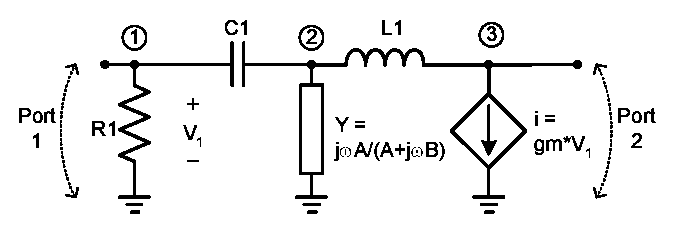
\includegraphics[scale=0.85]{Figures/Circuit.eps}
  \caption{Example circuit.}\label{fig:Circuit}
\end{figure}

Electrical circuits are entered into Milou by means of a
\emph{netlist} file, similar to the ones used in Spice. The
expressions shown in \tabref{Netlist} are recognized by the Milou
netlist parser:

\begin{table}[htbf]
    \centering
  \caption{Valid netlist expressions.}\label{tab:Netlist}
    \begin{minipage}{\textwidth}
    \centering
    \begin{small}
    \begin{tabular}{l|l}
    % after \\: \hline or \cline{col1-col2} \cline{col3-col4} ...
    Component & Netlist expression\\
    \hline
    Resistance & \verb"R value"\footnote{A \emph{value} can be either a numeric value or a parameter name.}\verb" node1 node2"\\
    Conductance & \verb"G value node1 node2"\\
    Capacitance & \verb"C value node1 node2"\\
    Inductance & \verb"L value node1 node2"\\
    General admittance & \verb"X expression"\footnote{An \emph{expression} can include an arbitrary algebraic expression. $s$ should be used instead of $j\omega$. Other names that are not recognized functions will be considered user parameters.} \verb" node1 node2"\\
    Transconductance& \verb"VCCS value node1+ node2+ node1- node2-"\\
    Transcond. with $\tau$& \verb"VCCSD value node1+ node2+ node1- node2-"\\
    Gyrator & \verb"GY value node1+ node2+ node1- node2-"\\
    General transcond. & \verb"X2 expression node1+ node2+ node1- node2-"\\
    Port & \verb"P portname node1 node 2"\\
    Comment & \verb"% Comment text" \\
    \hline
    \end{tabular}
    \end{small}
    \end{minipage}
\end{table}

The netlist corresponding to the circuit in \figref{Circuit}
becomes (\verb"circuit.net"):
\begin{small}
\begin{verbatim}
    % Example circuit
    R R1 1 0
    C C1 1 2
    X s*A/(A+s*B) 2 0
    L L1 2 3
    VCCS gm 1 3 0 0
    P P1 1 0
    P P2 3 0
\end{verbatim}
\end{small}

The netlist can now be imported into Milou by using the
\verb"read_netlist" function,
\begin{small}
\begin{verbatim}
    >> model = read_netlist(mna,'doc/Usersmanual/circuit.net')
    Admittance matrix:
        '+1/(R1)+s*C1'    '-s*C1'                 []
        '-s*C1'           [1x26 char]    '-1/(s*L1)'
        '+gm'             '-1/(s*L1)'    '+1/(s*L1)'
    Parameters:
        'R1'
        'C1'
        'A'
        'B'
        'L1'
        'gm'
    Parameter types:
        'R'
        'C'
        'X'
        'X'
        'L'
        'VCCS'
    Frequencies
    Partials
        1
        1
        1
        1
        1
        1
\end{verbatim}
\end{small}

The output variable \verb"model" is now an \verb"mna" object. mna
stands for \emph{modified nodal admittance}, which is the type of
matrix normally used to represent circuits in simulators. Milou
currently uses the ordinary nodal admittance matrix for
representing circuits\footnote{The modified nodal admittance
matrix uses a different representation of components that may
present infinite conductance, e.g. inductances at low frequency,
and thus provides better numerical stability.}. It is, by the way,
shown in the first part of the displayed \verb"mna" object
information displayed above.

The next thing displayed is the list of parameters. These are the
unique parameter names found in the netlist. The order in which
the parameters appear is important when, at a later stage, their
values should be assigned. The parameter names can also be
accessed by the \verb"params" command,
\begin{small}
\begin{verbatim}
    >> params(model)
    ans =
        'R1'    'C1'    'A'    'B'    'L1'    'gm'
\end{verbatim}
\end{small}

Next in the results displayed is the types associated with the parameters.
This is not applicable for parameters defined in \verb"X" or
\verb"X2" elements.

Finally, there is a list of partial derivatives that are used for
calculating sensitivities. This feature is, however, not treated
in this manual text.

\subsection{Evaluation of the model X-parameters}
Before it is possible to assign numbers to the model parameter and
evaluate its X-parameters, one needs to specify the frequencies
used for consequent calculations. The reason that the frequencies
are entered separately is to speed up the X-parameter evaluations
later. The frequencies are assigned to the \verb"mna"-object using
the \verb"freq" command,
\begin{small}
\begin{verbatim}
    >> model = freq(model,msp.freq);
\end{verbatim}
\end{small}
where the same frequencies as in the previous measurement examples
have been used.

It is now possible to evaluate the model for any set of parameters
using a call to either the \verb"calc" or the \verb"reduce"
functions. The model parameter values should be arranged in a
vector with the order being the same as described above.
\begin{small}
\begin{verbatim}
    >> R1 = 100;C1 = 1e-12;A = 0.7e-12;B = 2e-12;
    >> L1 = 1e-9; gm = 1e-3;
    >> model_params = [R1,C1,A,B,L1,gm];
\end{verbatim}
\end{small}

Once the parameters have been defined it is possible to calculate
either the full $N$-by-$N$ matrix, where $N$ is the number of
nodes, or a reduced matrix describing the circuit as observed at
the ports that were defined in the netlist.

The first case is evaluated by using the \verb"calc" function,
\begin{small}
\begin{verbatim}
    >> calc(model,model_params)
    xparam-object
        type:  Y
        reference: 50
        ports: 3
        elements:  101
\end{verbatim}
\end{small}
The resulting object is, for our three-node example a 3-by-3
Y-type \verb"xparam" object.

The function \verb"reduce" is used in a similar fashion to
calculate the port-reduced Z-parameters,
\begin{small}
\begin{verbatim}
    >> xp_model = reduce(model,model_params)
    xparam-object
        type:  Z
        reference: 50
        ports: 2
        elements:  101
\end{verbatim}
\end{small}
Note that the resulting object is a 2-by-2 Z-type \verb"xparam"
object, which can be handled in exactly the same manner as the
measurements were used before.

% $Header$
% $Author: fager $
% $Date: 2009-04-28 20:51:04 +0200 (ti, 28 apr 2009) $
% $Revision: 99 $
% $Log$
% Revision 1.3  2005/02/22 07:31:00  fager
% Corrections from M.Kelly implemented
%
% Revision 1.2  2004/10/21 18:59:06  fager
% Version logging added. Comments from KA implemented.
%

\section{Sweeps of measurements}\label{sec:sweeps}
MuWave has not only functionality to handle single measurements,
using the \verb"meassp" class, but also a series of measurements.
Typically, this is a series of measurements obtained at different
bias points. The class used to handle these swept measurements is
called \verb"meassweep".

MuWave can create \verb"meassweep" objects from either a directory
with multiple TouchStone files or from an MDIF file\footnote{See
Agilent ADS documentation for details about the MDIF file
format.}.

\subsection{Importing multiple Touchstone files}
Multiple TouchStone files are imported into an \verb"meassweep"
object using the function \verb"read_milousweep". The following
example shows a typical call with this function:
\begin{small}
\begin{verbatim}
    >> sweep = read_milousweep(meassweep,...
    Measurement info
        Date : 14-Apr-2009 10:54:07
        Origin : muwave\test\d0509_all\d0506_*
        Operator :
        Info :
    Sweep info
    	Vgs,min: -0.5
    	Vgs,max: 0.2
    	Vds,min: 0.5
    	Vds,max: 1.5
    	Igs,min: -7.94141e-007
    	Igs,max: 2.05474e-006
    	Ids,min: 0.00343814
    	Ids,max: 0.0297255
    	Number of measurements: 24
\end{verbatim}
\end{small}
Please consult \verb">> help read_milousweep" to find the details
on how to call this function.

\subsection{Importing MDIF-files}
MDIF files allow a convenient way of transferring multi
dimensional data to and from Agilent ADS. The structure of the
MDIF files are described in the Agilent ADS manual and not
repeated here.

The function \verb"read_mdif" can be used to import MDIF data into
a \verb"meassweep" object in Milou. It should be stressed that, at
the time of writing, this function is still under development and
may not operate as expected!

\subsection{Importing Maury ATS swept bias S-parameters}
The function \verb"read_s2b" allows Milou to import swept bias
S-parameter files created by the Maury Microwave ATS software.
Please consult the on-line help for more information about this
function.

\subsection{Accessing and indexing meassweep objects}
A \verb"meassweep" object can thought of as a vector of
\verb"meassp" objects. An individual \verb"meassweep" object, or a
subset of the \verb"meassweep" can be accessed using the
parenthesis \verb"()" operator,
\begin{small}
\begin{verbatim}
    >> sweep(1)
    Measurement info
        Date : 2002-10-24, 19:23
        Origin : muwave\test\d0509_all\d0506_0
        Operator :
        Info :
    Measurement state
    	MeasType:	SP
    	Vgs:	-0.5
    	Vds:	0.5
    	Igs:	-6.43067e-007
    	Ids:	0.00343814
    xparam-object
    	 type:	S
    	 reference:	50
    	 ports:	2
    	 elements:	101
    	 freq:	1E+009 -> 5E+010
    >> sweep(1:10)
    Measurement info
        Date : 14-Apr-2009 10:54:07
        Origin : muwave\test\d0509_all\d0506_*
        Operator :
        Info :
    Sweep info
    	Vgs,min: -0.5
    	Vgs,max: 0.2
    	Vds,min: 0.5
    	Vds,max: 1
    	Igs,min: -6.97489e-007
    	Igs,max: 7.27892e-007
    	Ids,min: 0.00343814
    	Ids,max: 0.0233942
    	Number of measurements: 10
\end{verbatim}
\end{small}

\subsection{The dot-operator}
An individual parameter of the sweep objects can be accessed using
the dot-operator. The following example shows how to access the
\verb"Vgs"-parameter and also how this can be used to use reduce
the sweep-object to contain only bias points with \verb"Vgs" $=0$.
\begin{small}
\begin{verbatim}
    >> sweep.Vgs
    ans =
    Columns 1 through 7
    -0.5000   -0.4000   -0.3000   -0.2000   -0.1000   -0.0000    0.1000
    Columns 8 through 14
        0.2000   -0.5000   -0.4000   -0.3000   -0.2000   -0.1000   -0.0000
    ...

    >> bias_index = find(abs(sweep.Vgs)<0.01);
    >> sweep(bias_index)
    Measurement info
        Date : 14-Apr-2009 10:54:07
        Origin : muwave\test\d0509_all\d0506_*
        Operator :
        Info :
    Sweep info
    	Vgs: -2.77556e-017
    	Vds,min: 0.5
    	Vds,max: 1.5
    	Igs,min: -1.09436e-007
    	Igs,max: -4.34143e-008
    	Ids,min: 0.0212195
    	Ids,max: 0.0257597
    	Number of measurements: 3
\end{verbatim}
\end{small}

\subsection{Adding measurements}
Single measurements can be added to the \verb"meassweep" object
with the \verb"add" function,

\begin{small}
\begin{verbatim}
    >> msp = read_touchstone(meassp,'muwave\test\d0509\d0509_20');
    >> sweep_total = add(sweep,msp);
    >> length(sweep_total)-length(sweep)
    ans =
        1
\end{verbatim}
\end{small}
The same function, \verb"add", can also be used to merge two
\verb"meassweep" objects.

\subsection{Writing swept data}
For the moment, no functions have been implemented to write a
\verb"meassweep" object to multiple TouchStone files or into an
MDIF-file.

% $Header$
% $Author: fager $
% $Date: 2004-10-21 20:59:19 +0200 (Thu, 21 Oct 2004) $
% $Revision: 223 $
% $Log$
% Revision 1.2  2004/10/21 18:59:06  fager
% Version logging added. Comments from KA implemented.
%

\section{Plotting functions}
Finally, some useful functions for plotting \verb"meassp" and
\verb"meassweep" data are described.

\subsection{Combined Smith/polar diagram}
A combined Smith/polar diagram for depicting two-port S-parameters
is easily produced with the \verb"smithplot" function. It takes a
\verb"meassp" object as input and generates a combined Smith/polar
plot for all four S-parameters (See \figref{Smith}):
\begin{small}
\begin{verbatim}
    >> smithplot(msp);
\end{verbatim}
\end{small}

\begin{figure}[htbf]
    \centering
  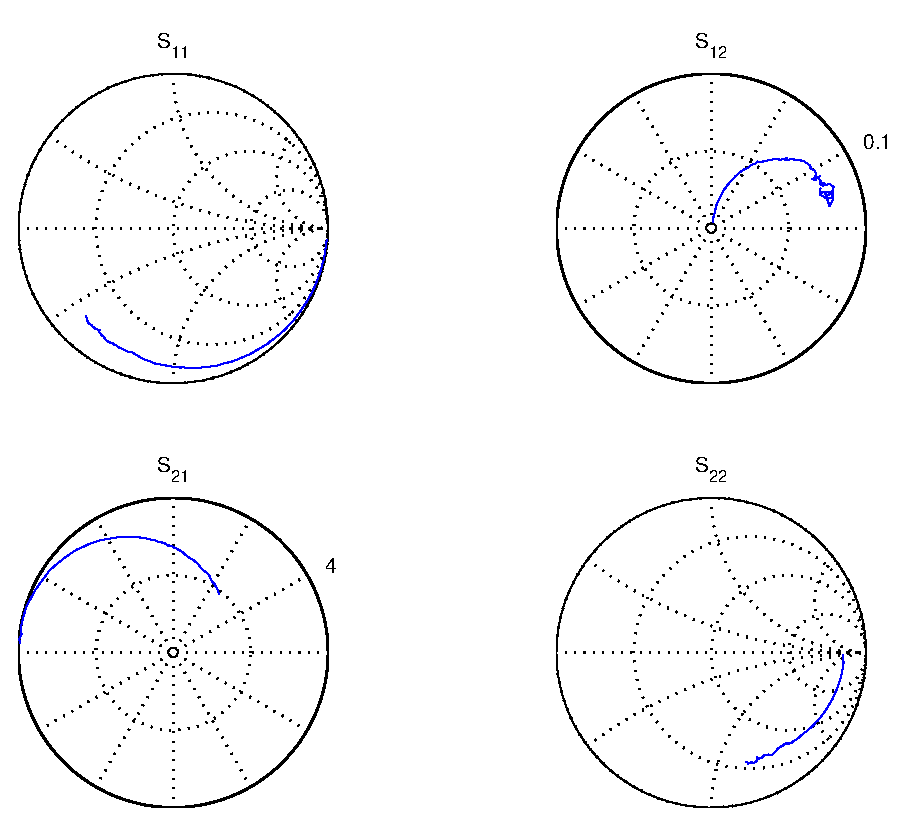
\includegraphics[scale=0.6]{Figures/Smith.eps}
  \caption{Combined Smith/polar diagram produced with smithplot.}\label{fig:Smith}
\end{figure}

\subsection{Single parameter plot}
Single parameters may be plotted using the \verb"paramplot"
command. It is particularly useful for producing single parameter
Smith plots. The syntax for this is given below.
\begin{small}
\begin{verbatim}
    >> paramplot(msp,'S11','smith',gca);
\end{verbatim}
\end{small}
Other plotting methods are available as described in the help at
\newline \verb">> help paramplot".

\subsection{Swept data}
A modified \verb"plot" function has been implemented to plot
parameters of \verb"meassweep" object against each other. This is
useful for producing I/V plots from the biasing information
contained in the measurement files. The syntax is exemplified by,
\begin{small}
\begin{verbatim}
    >> plot(sweep,'Vgs','Ids')
\end{verbatim}
\end{small}
The plot produced is shown in \figref{IdsVgs}.

\begin{figure}[htbf]
    \centering
  \includegraphics[scale=0.6]{Figures/IdsVgs.eps}
  \caption{Ids-Vgs characteristics produced with the meassweep-plot function.}\label{fig:IdsVgs}
\end{figure}

\end{document}
